\section{OGLE IV classical Cepheids on the Magellanic clouds}

\subsection{The OGLE project}

The Optical Gravitational Lensing Experiment (OGLE) project is an earth-based observational astronomical project 
with the objective of study dark matter and microlensing phenomena in the Magellanic clouds and the Galactic bulge.
This project was originated by an idea of Bohdan \cite{Paczynski1986}. 
Its first phase began in 1992, with very limited time in the 1m Swope telescope, in Las Campanas Observatory, Chile,
operated by the Carnegie Institution of Washington.

Those initial observation continued until 1995, and produced many interesting results: 
apart from its initial goal of observing microlensing events \citep{Udalski1993},
they published extinction maps of the galactic bulge \citep{Stanek1996},
and the first version of their catalog of variable stars \citep{Udalski1997}.

The whole idea of Paczyński was a great success despite its difficulties,
and therefore the Warsaw University decided to further fund OGLE.
In 1995 began the construction of the 1.3m Warsaw telescope and observing site at the same observatory, due to its optimal position.
The construction, assembly and tests were concluded by late 1996, 
and in 1997 began the second phase of the project.

Third and fourth OGLE phases began in 2001 and 2010 respectively. 
The last phase, OGLE-IV, is still on pause at the time of writing this document (late 2021) due to the COVID-19 pandemic.
As of 2019, their main site\footnote{\url{http://ogle.astrouw.edu.pl/}} reported $\sim$800 papers published from the main OGLE results,
and $\sim$1300 OGLE-related results. 
All of that makes the OGLE project one of the oldest observational projects that have been focused on the same objects,
making it an invaluable resource for studying the Magellanic system and the galactic bulge.

\begin{table}
	\centering
	\begin{tabular}{l|rrrrrrr}
		mode &     stars &  with I & only I & with V & only V & both &  none \\ \hline\hline
		F      &  2477 &  2428 &       151 &  2287 &        10 &  2277 &    39 \\
		1O     &  1776 &  1766 &       116 &  1650 &         0 &  1650 &    10 \\
		2O     &    26 &    26 &         0 &    26 &         0 &    26 &     0 \\
		F1O    &    95 &    95 &         6 &    89 &         0 &    89 &     0 \\
		1O2O   &   322 &   321 &        16 &   305 &         0 &   305 &     1 \\
		F1O2O  &     1 &     1 &         0 &     1 &         0 &     1 &     0 \\
		1O2O3O &     7 &     7 &         0 &     7 &         0 &     7 &     0 \\
		1O3O   &     1 &     1 &         0 &     1 &         0 &     1 &     0 \\
		2O3O   &     1 &     1 &         0 &     1 &         0 &     1 &     0 \\\hline
		total  &  4706 &  4646 &       289 &  4367 &        10 &  4357 &    50 \\
		\end{tabular}
		\caption[Pulsation mode and filter data distribution for the LMC]{
			Distribution of the number of stars in the database for the LMC according with their reported pulsation mode.
			The first column give the total of stars in that mode.
			The next four columns give how many of those stars have data in $I$ band, \textit{only} $I$ band, and the same for $V$ band.
			The last two columns enumerates the stars that have data in both bands and the stars of which no data were found in the database.
			As can be seen, there are so few stars with pulsation modes F1O2O, 1O2O3O, 1O3O, and 2O3O, 
			that their inclusion in the following analysis would be less than satisfactory.
		}
		\label{tab:LMC}
\end{table}

\begin{table}
	\centering
	\begin{tabular}{l|rrrrrrr}
		mode &     stars &  with I & only I & with V & only V & both &  none \\ \hline\hline
		F      &  2754 &  2739 &       125 &  2617 &         3 &  2614 &    12 \\
		1O     &  1791 &  1783 &        86 &  1697 &         0 &  1697 &     8 \\
		2O     &    91 &    91 &         2 &    89 &         0 &    89 &     0 \\
		F1O    &    68 &    68 &         2 &    66 &         0 &    66 &     0 \\
		1O2O   &   239 &   239 &         9 &   230 &         0 &   230 &     0 \\
		1O2O3O &     1 &     1 &         0 &     1 &         0 &     1 &     0 \\\hline
		total  &  4944 &  4921 &       224 &  4700 &         3 &  4697 &    20 \\
	\end{tabular}
	\caption[Pulsation mode and filter data distribution for the LMC]{
		Same as \autoref{tab:LMC} but for the SMC. 
		This time, there is a single star with pulsation mode 1O2O3O,
		and therefore it will be excluded from the analysis.
		This choice leaves the LMC and the SMC with the same pulsation categories.
	}
	\label{tab:SMC}
\end{table}

\subsection{Data acquisition and description \label{sec:data}}

% instrumentation

As previously mentioned, the OGLE project uses its own 1.3m telescope at Las Campanas Observatory, Chile,
fully described by \cite{OGLEIIinstrumentation}. 
The OGLE-IV phase uses this telescope, and since 2009 they use a mosaic camera of 32 thin E2V44-82 2048×4096 CCD chips,
with 0.26 arcsec/pixel scale and 1.4 square degrees total field of view.
The whole data obtention process, the specific mosaic arrangement and the sky coverage are described by \cite{OGLE2015}.

% description

This work uses a subset of the The Ogle Catalog of Variable Stars (OCVS), publicly available to download for the 
astronomic community at \url{http://www.astrouw.edu.pl/ogle/ogle4/OCVS/}.
Specifically, we will use the photometric data from Classical Cepheids in the Small and Large Magellanic clouds (SMC,LMC).
This section of the catalog is composed of 9583 individual stars, with data on the $I$ and $V$ magnitude, 
taken with the filters shown in \autoref{fig:filters}, but converted to the standard Johnson-Cousins photometric system \citep{OGLE2015}.
Each data file is composed of three columns, the date of the observation in $RHJD=HJD-2.45\times 10^6$, 
the measured magnitude, and its uncertainty. 
Uncertainties though the data varies from $0.004$ mag to $0.1$ mag in the most extreme cases. 
Those cases are extremely rare, however, and the mean stays at around $0.006$ mag.

% missing data and tables

There are some stars that, perhaps by observation schedule, perhaps by reclassification, have no data files in some filters, or have data in only one.
This information, separated by reported pulsation mode, is detailed in \autoref{tab:LMC} for the LMC and in \autoref{tab:SMC} for the SMC.
The stars with no data will be ignored, as well as the rarest pulsation modes.
From those tables is clear that stars with $I$ magnitude data are slightly more prevalent.
In fact, even for a star that has data in both filters, there is usually a lot more $I$ magnitude observation than $V$ ones.
The distribution of data points per star per filter can be seen in \autoref{fig:n-hist}.
Probably the $V$ data was only taken to measure its mean, in order to construct the Wesenheit index,
while the $I$ data was taken both for the mean $I$ magnitude and to calculate the period.

\begin{figure}
	\centering
	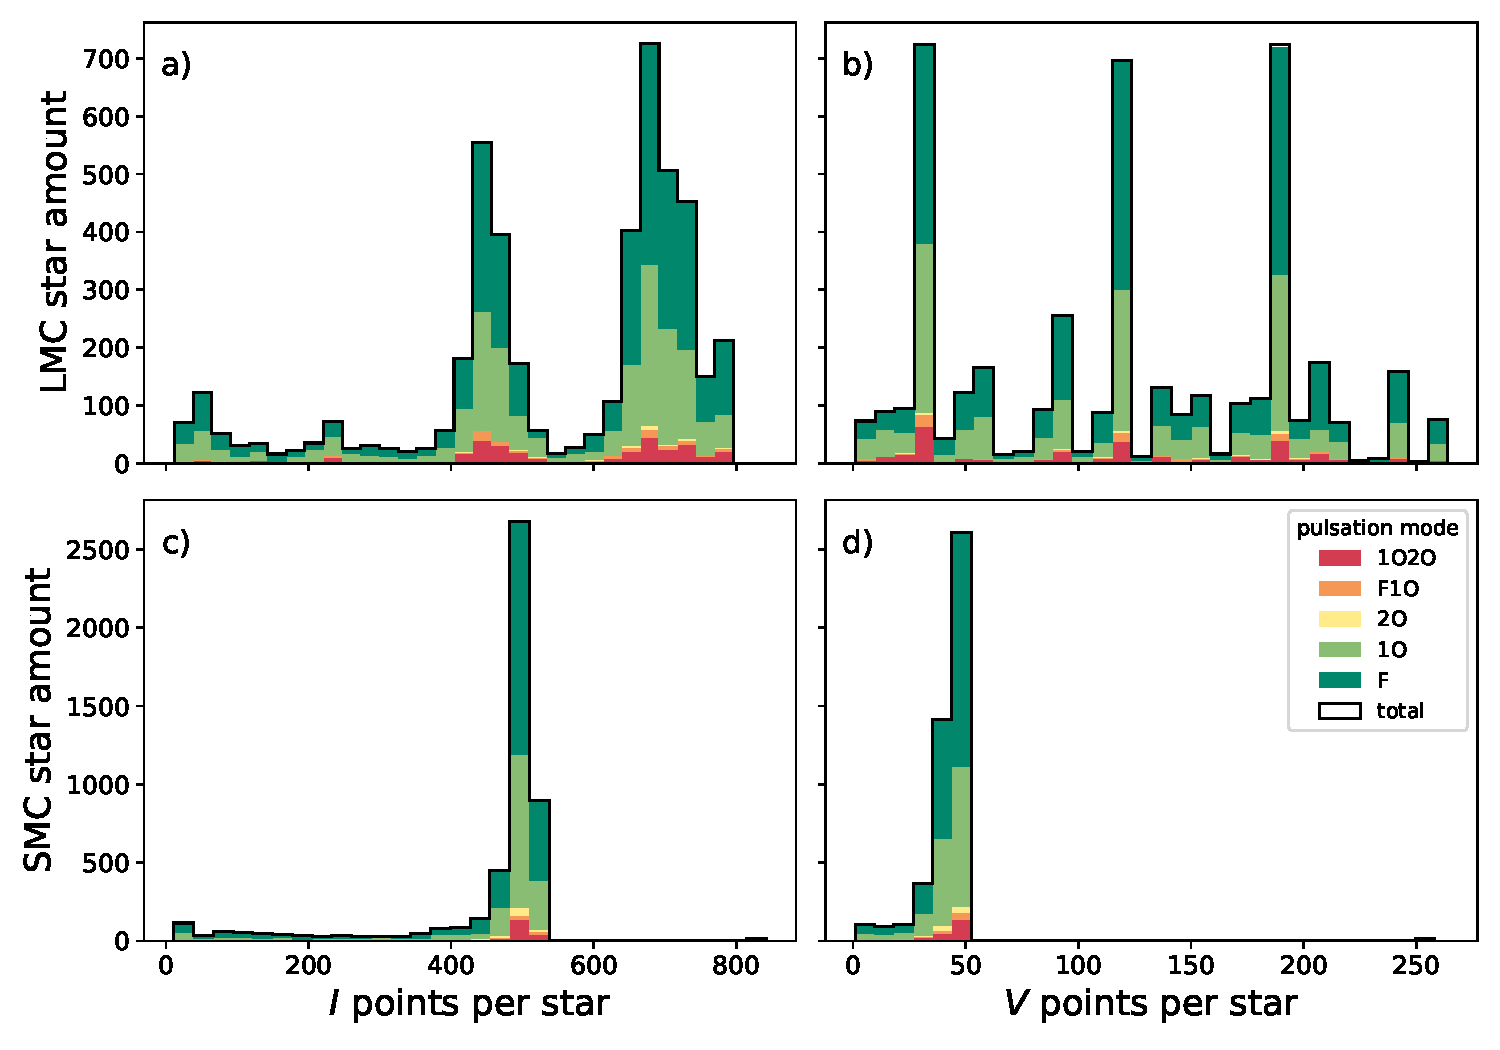
\includegraphics[width=0.9\textwidth]{img/clouds_histogram_ns.pdf}
	\caption[Distribution of data size for classical Cepheids in the Magellanic clouds]{
		Distribution of data points per star in both $I$ and $V$ filters for the LMC and the SMC. 
		Histograms are cumulative, and each color represents the contribution fraction of each pulsation mode on each bin.
		Total is outlined in black.
		As expected, there are much more data points in the LMC compared to the SMC due to their size difference.
		There is also much more data in $I$ magnitude, as outlined in the text.
		The threshold for minimum number of points required by the period finding algorithms is around 50,
		which made the $V$ data unusable for finding periods on the SMC case (d).
		If only $I$ data is to be used for this purpose, 
		the lower tails on both clouds can be cut at around ~400 points without loosing too many stars.
	}
	\label{fig:n-hist}
\end{figure}


% data distributions

In order to define our frequency grid for the period search, the OGLE reported periods can be examined to deduce a reasonable range.
The distributions of $I$ mean magnitude and amplitude can also be examined, as they are all presented in \autoref{fig:pidi-hist}.
There one can see some bimodal behaviors with small tails in the long-period high-luminosity end of the data, 
and sometimes a distinction between the pulsation modes can be made.

\begin{figure}
	\centering
	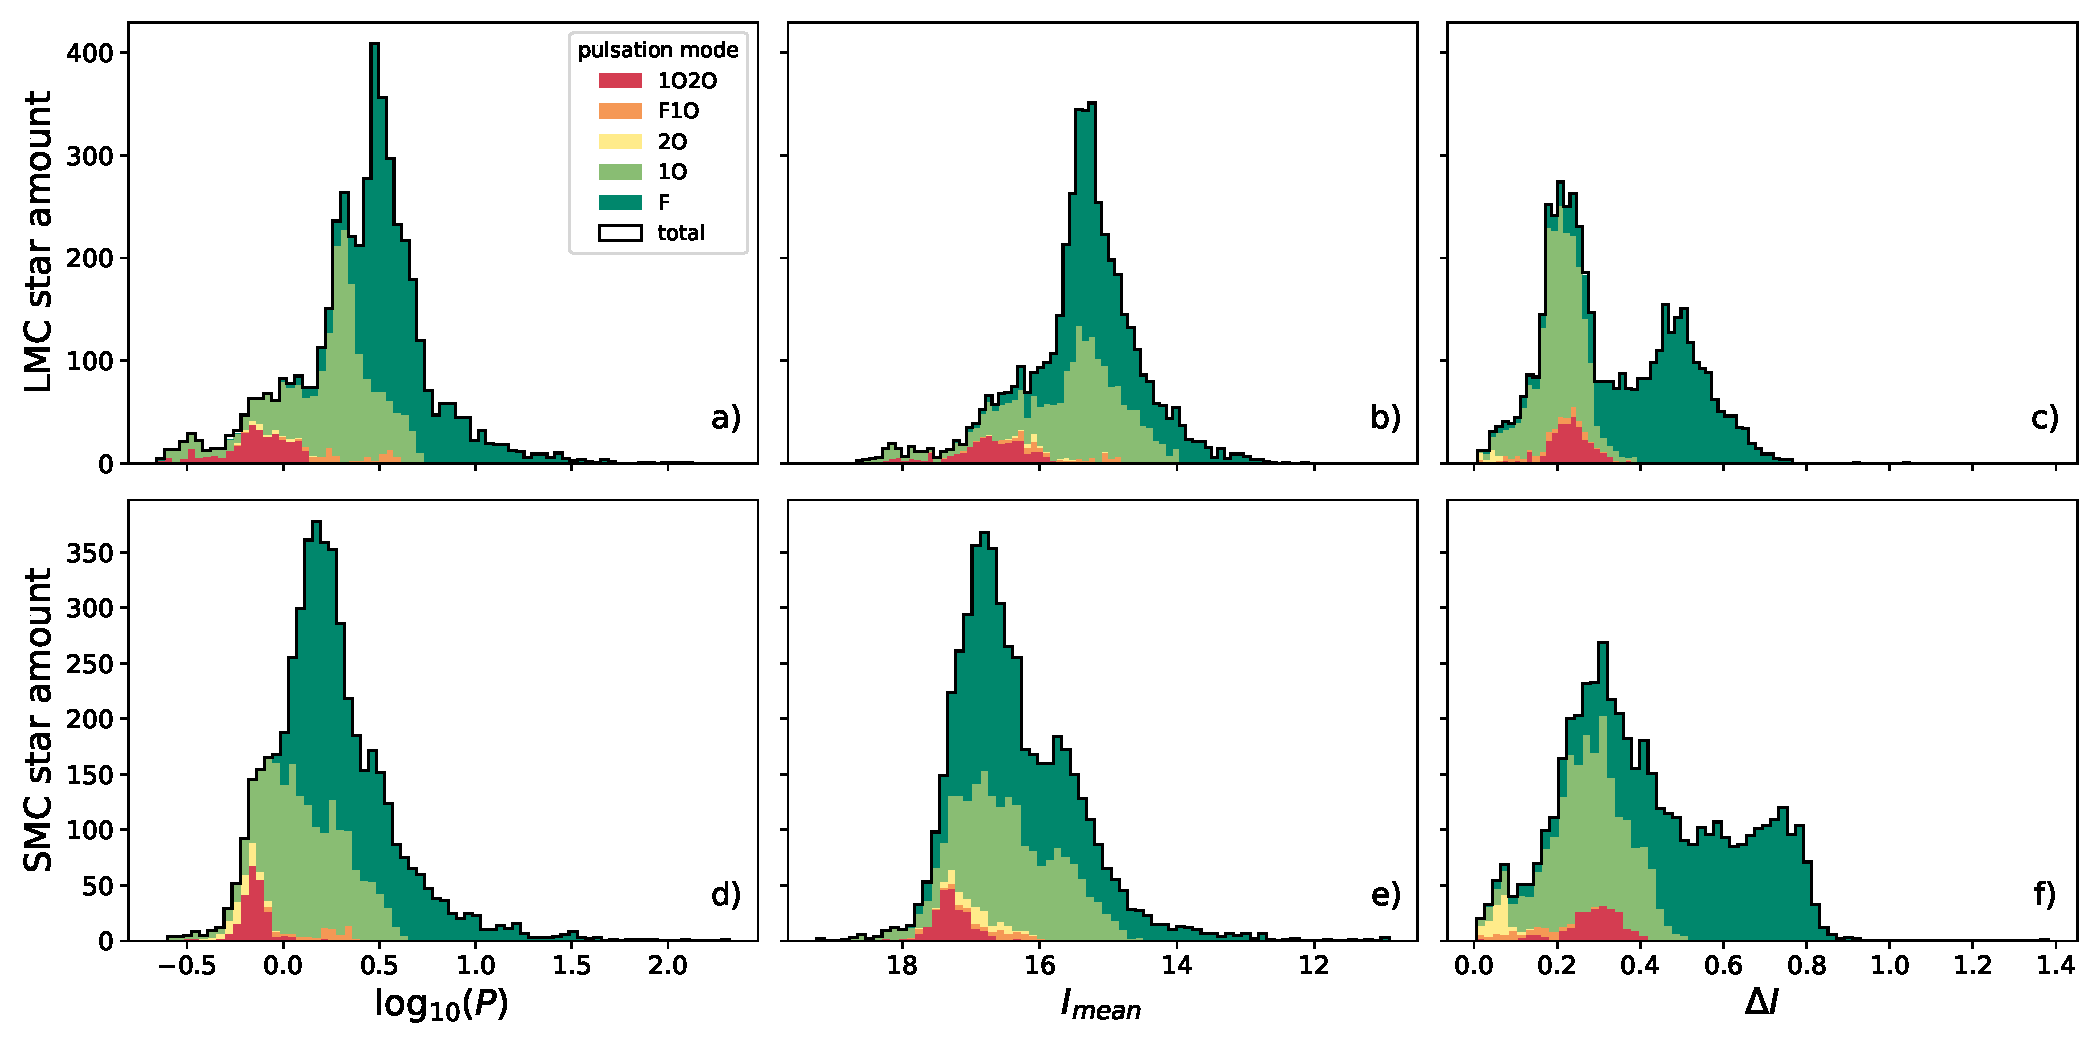
\includegraphics[width=\textwidth]{img/clouds_histogram_PIdI.pdf}
	\caption[Distribution of signal properties for classical Cepheids in the Magellanic clouds]{
		Distribution of periods, mean $I$ magnitudes and $I$ amplitudes for the OGLE classical Cepheids in the Magellanic system.
		Histograms are cumulative, and each color represents the contribution fraction of each pulsation mode on each bin.
		Total is outlined in black.
		In the case of multi-period stars, only the lower one is considered, as reported in the data headers \texttt{*.cep}.
		The tails on the longer periods and brightest and widest stars are kept in the plot range, despite having so few stars,
		to represent the difficulty of studying the bright side of the PL relation.
	}
	\label{fig:pidi-hist}
\end{figure}

% temporal cadence

\subsubsection{Sampling and observation cadence \label{sec:sampling}}

All of these observations are made on earth, and as such,
they are limited to the sky conditions, tight scheduling and the earth rotation.
Therefore, the cadence of observations is far from being evenly sampled.
An example of this uneven nature of the data is presented on \autoref{fig:1234-cadence} for a single star,
and on \autoref{fig:global-cadence} for the whole of OGLE-IV measurements.

As we are not interested in signal reconstruction, but only in finding the true period,
we can bypass the mean sampling frequency limit given by \cite{Marvasti2001}.
In theory, when a signal is evenly sampled, one could only calculate its periodogram up to half that frequency (the Nyquist frequency);
all the subsequent peaks are false peaks, reflections of the spectrum. 
An example of this can be seen on \autoref{fig:uneven-advantage}.

The is shown how uneven sampling might be even beneficial, as one can freely search for a frequency much higher that 
the mean Nyquist limit for the data. How much this effect lasts and hwy many points does it need to be useful remains to bee seen.

\begin{figure}
	\centering
	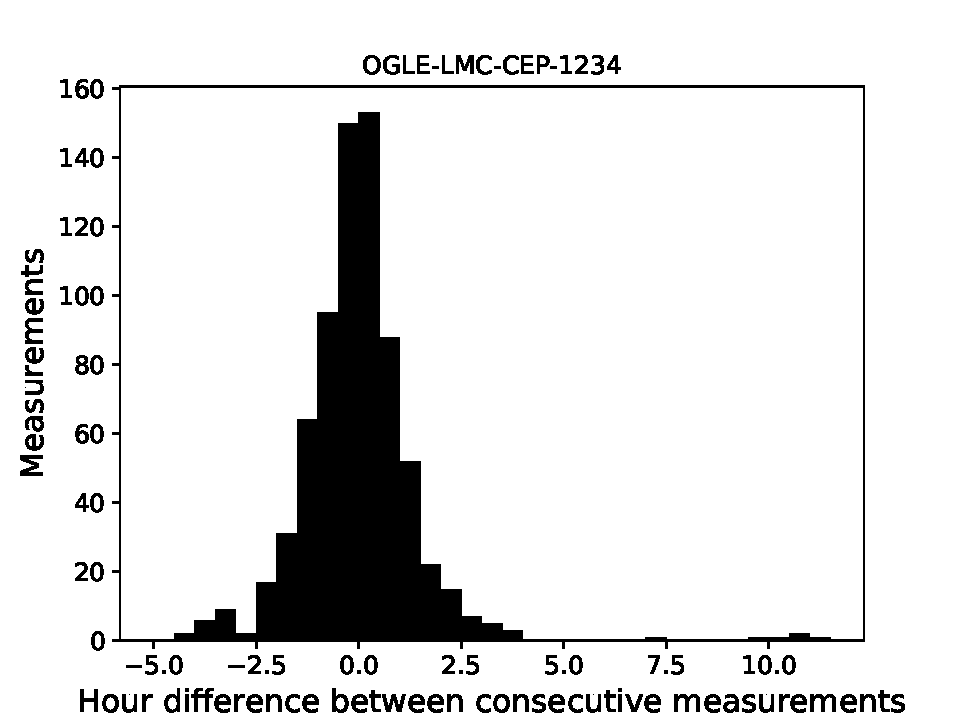
\includegraphics[width=0.5\textwidth]{img/1234_cadence.pdf}
	\caption[Hourly difference between observations for OGLE-LMC-CEP-1234]{
		Histogram of the \textit{hour} difference between consecutive observations for a sample star in the LMC.
		This hour difference is defined as the time difference modulo one day; 
		for example, if one observation was made on Monday at 1:00am, and the next on Tuesday at 3:00am, the hour difference would be 3.
		The small clump on $\sim$10 hours is due to the yearly pauses on observations, as can be seen on Figures \ref{fig:mag-phase-1} and \ref{fig:mag-phase-2}.
		If the data were to be evenly sampled, this histogram would look like a delta function.
	}
	\label{fig:1234-cadence}
\end{figure}


\begin{figure}
	\centering
	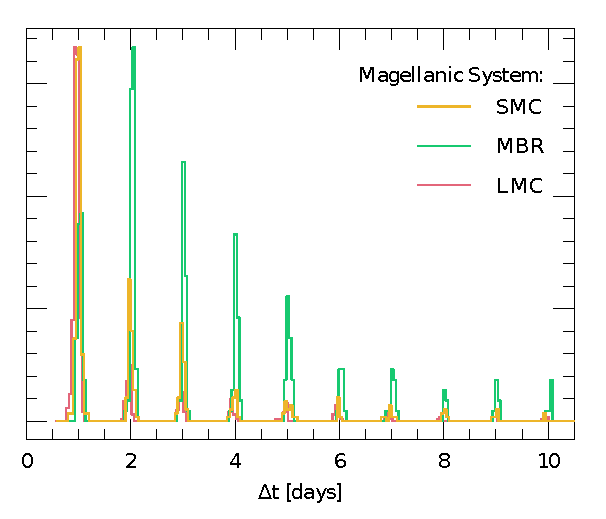
\includegraphics[width=0.45\textwidth]{img/fig_19_65_1_1.pdf}
	\caption[OGLE-IV observation cadence in the Magellanic system]{
		Histogram of the time difference between consecutive observations on OGLE-IV, for the clouds (LMC, SMC) and the Magellanic Bridge (MBR).
		\autoref{fig:1234-cadence} is basically a phase diagram of the LMC histogram, 
		but only considering the observations made to one star.
		The vertical scale is normalized to the highest point of each curve.
		Taken from \cite{OGLE2015}, Figure 19.
	}
	\label{fig:global-cadence}
\end{figure}

\section{Implementation details}

All of the algorithms presented here are programmed in Python \citep{VanRossum2009} for simplicity,
but with extensive use of the NumPy \citep{vanderWalt2011} and Numba \citep{Lam2015} libraries to achieve greater performance.

No claim is made that these algorithms are optimal, 
but effort was putted on implement the optimizations commonly used in the literature.

All of the algorithms take a time array, a magnitude array, and a frequency array as parameters.
The minimum entropy and minimum dispersion algorithms also take an integer number of bins.

\subsection{Algorithms}

\subsubsection{Arclength}

For each frequency in the search array:

\begin{itemize}
	\item \autoref{lst:phase} is used to calculate the phase with the time and magnitude arrays.
	\item The phase array is sorted, and the magnitude array is rearranged accordingly.
	\item The differences between contiguous phases and magnitudes are calculated.
	\item Those differences are squared and then added, according to \autoref{eq:arclength}
	\item Optionally, the square root is taken. This does not affect the peaks except by a scaling.
	\item The total sum is returned as the arclength.
\end{itemize}

The best guess for the correct frequency would be where the arclength is minimum.
A possible implementation of a single iteration of the method is given in \autoref{lst:arclength}.

\subsubsection{Entropy}

For each frequency in the search array:

\begin{itemize}
	\item \autoref{lst:phase} is used to calculate the phase.
	\item A binning algorithm, like \autoref{lst:hist2d}, is used to calculate a 2D histogram of the phase diagram.
	\item The histogram counts are transformed in the probabilities $\mu_j$ of \autoref{eq:entropy}.
	\item The zero probability bins are deleted, to avoid a numerical error taking the logarithm.
	\item The sum on \autoref{eq:entropy} is returned as the entropy.
\end{itemize}

The best guess for the correct frequency would be where the entropy is minimum.
A possible implementation of an iteration is given in \autoref{lst:entropy}.

A big improvement can be made by translating the phase-magnitude plane $\{\phi_k,m_k\}$ into a line $\lfloor m_k n_{bins} \rfloor + \phi_k$,
analogous at making the phase \enquote{tens} and the phase \enquote{units}.
Over that transformed line, a 1D histogram algorithm can be used with $n_{bins}^2$ number of bins, hence the phase diagram is \enquote{flattened}. 
That implementation is given in \autoref{lst:entropy-flattened}. 
This flattening allows the use of very efficient 1D binning algorithms.

\subsubsection{Dispersion}

For each frequency in the search array:
\begin{itemize}
	\item \autoref{lst:phase} is used to calculate the phase.
	\item For each uniform zone (partition of the phase $[0,1]$ range), 
	calculate the occupation number and the variance of the magnitudes corresponding to the phases on the zone.
	\begin{itemize}
		\item If the zone is empty, the variance is defined as zero. This makes some sense because the (biased) variance 
		$\frac{\sum(x-\bar{x})^2}{n}$ would be an empty sum with a second order zero in the numerator and a first order zero in the denominator.
	\end{itemize}
	\item The pooled variance $s^2$ of all the zones is calculated with \autoref{eq:pooled-variance}. 
	The overall variance $\sigma^2$ is just the variance of all the magnitudes.
	\item The coefficient of determination $R^2=1-s^2/\sigma^2$ is returned as the dispersion.
\end{itemize}

The best guess for the correct frequency would be where this $R^2$ is maximum.
This $R^2$ approximates really well the Fourier spectrum, as can be seen in \autoref{fig:examples}.
The implementation is in \autoref{lst:dispersion}

\subsubsection{Lomb-Scargle}


The original formulas for the Lomb-Scargle periodogram (Equations \ref{eq:lomb-scargle} and \ref{eq:tau}) 
involve several redundant trigonometric calculations.
Here we implement the optimizations given by \cite{Townsend2010}, where no trigonometric function is repeated.

For each frequency $\nu$ in the search array, being $t$ the time array and $m$ the magnitude array:
\begin{itemize}
	\item Calculate:
	\begin{itemize}
		\item $\omega t = 2\pi\nu t$
		\item $C=\cos\omega t$
		\item $S=\sin\omega t$
		\item $mC= m \cdot C$
		\item $mS = m \cdot S$ 
		\item $CC=C\cdot C$
		\item $SS=S\cdot S$
		\item $CS=C \cdot S$
		\item $\omega\tau = \frac12 \arctan\left(\frac{2 CS}{CC-SS}\right)$
		\item $c_\tau = \cos\omega\tau$
		\item $s_\tau = \sin\omega\tau$
	\end{itemize}
	\item return the coefficient of determination
	$$
	R^2 = \frac12 \left(\frac{(c_\tau mC + s_\tau mS)^2}{c_\tau^2 CC + 2 c_\tau s_\tau CS + s_\tau^2 SS}
	+ \frac{(c_\tau mS-s_\tau mC)^2}{c_\tau^2 SS + 2 c_\tau s_\tau CS + s_\tau^2 CC}\right).
	$$
\end{itemize}

As before, the correct frequency is at maximum $R^2$, and this is also a good approximation of the Fourier spectrum.

\subsubsection{Fourier}

A straightforward calculation of \autoref{eq:fourier} would actually be enough to outperform some (if not all) of the aforementioned methods,
but there is an iterative optimization provided by \cite{Kurtz1985}, that calculates the transform on the next frequency modifying the last calculation,
saving a lot of time.

Thus, contrary to all the other methods, this implementation cannot be putted into a single-iteration function.
Also contrary to the other methods, it requires the frequency grid to be evenly spaced. This is not a problem, 
as the only problem were the \textit{times} to be unevenly spaced.
Additionally, if we have no idea of the correct frequency in the first place, 
there is no worse nor better way to search for it than in an evenly spaced frequency grid.

The idea behind this optimization is that if the frequencies are of the form $\nu_j = \nu_{j-1} + \Delta \nu$, the centroid from \autoref{eq:centroid} 
can be written (element-wise) as
\begin{equation}
	C(\nu_j)_k = f_k e^{2i\pi (\nu_{j-1}+\Delta \nu) t_k} = f_k e^{2i\pi \nu_{j-1} t_k} e^{2i\pi \Delta \nu t_k} = C(\nu_{j-1})_k e^{2i\pi \Delta \nu t_k},
\end{equation}
where $j$ goes over the frequencies and $k$ over times/magnitudes. 
The array $D_k = e^{2i\pi \Delta \nu t_k}$ is constant, 
so the coordinates of the \enquote{curled object} in the complex plane that we took the centroid off (see \autoref{fig:complex-phase-off})
for a certain frequency, can be calculated from the last coordinates by just multiplying element-wise by $D$.

Given $\nu_0,\nu_f,\Delta \nu$, the time array $t_k$ and the magnitude array $f_k$, the algorithm would look like:

\begin{enumerate}
	\item Calculate $D_k = e^{2i\pi \Delta \nu t_k}$
	\item Allocate an array $F_k$ of the same size as the frequency range, $J=\lfloor \frac{\nu_f-\nu_0}{\Delta \nu} \rfloor$, to store the centroid magnitudes.
	\item Initialize $\nu=\nu_0$.
	\item Calculate the first \enquote{curled object} in the complex plane, $C_k = f_k e^{2i\pi \nu_0 t_k}$.
	\item Initialize $F_0 = \left|\sum_k C_k\right|^2$
	\item While $\nu<\nu_f$, or equivalently, for $j \in [1,J]$
	\begin{itemize}
		\item $C_k \to C_k \star D_k $, where $\star$ means element-wise multiplication
		\item $F_j \to \left|\sum_k C_k\right|^2$
	\end{itemize}
	\item Return $\nu_k = \nu_0 + k \Delta \nu$ where $F_k$ is maximum. 
\end{enumerate}

Perhaps the code on \autoref{lst:fourier} would be clearer.

\subsection{Examples and the sampling problem \label{sec:examples-and-aliases}}

A simple benchmark of the algorithms can be seen on \autoref{fig:runtimes}. 
It is of note that the minimum entropy algorithm (on the naive implementation) was the slowest, 
and the simple Fourier method was the fastest by far, even without optimizations.
The \enquote{flattened} implementation of minimum entropy (on red) is faster than de dispersion one, because the $M^2$ term in the 
$O(nM^2)$ complexity of the entropy calculation is generally small, and there is no linear term on counting bins in the histogram.
On the other side, despite the $O(nM)$ complexity of the dispersion method, each iteration contains variances and counting in addition to the tally,
so there is linear overhead on $n$.
The full spectrum iterative Fourier method has complexity $O(nf)$, with $f$ the number of frequencies.
It is slower than the $O(n \ln n)$, as for our purposes $f\gg n$.
Even with this, the incremental Fourier method seems to be the fastest on uneven sampled data.

Examples of the spectra produced by each method are in \autoref{fig:examples}.
As expected, the Lomb-Scargle and dispersion spectra are very good approximations of the pure Fourier one.
Of course, there are some random noise and minor peaks that make those three differ, and even more with the arclength spectrum.
The entropy spectrum is the most different, considering that the peak is sharper 
(in the first star) and it present false peaks at $\nu\approx 1$/day\footnote{
	It's never exactly 1/day, because of the peak on \autoref{fig:1234-cadence}. 
	The earth moves around the sun, and optimal observing times also move.
	Then the peak will not be exactly at zero.
}. In fact, the Fourier methods also present that peaks, but they can be eliminated.

\begin{figure}
	\centering
	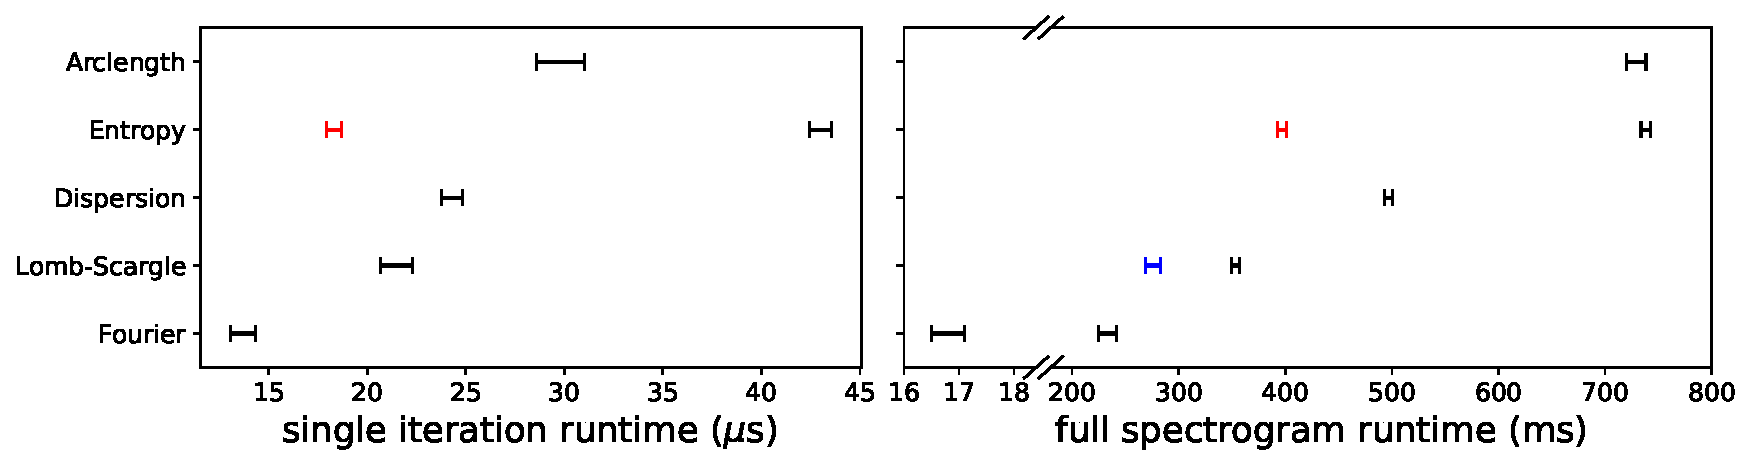
\includegraphics[width=\textwidth]{img/runtimes.pdf}
	\caption[Illustrative benchmark for the algorithms]{
		Sample benchmark of repeated single-threaded runs over all the algorithms described in this section.
		The single iteration times were calculated with 50000 repetitions of 7 runs, 
		and the full spectrum times were made on a regular frequency grid of size 14000, with 10 repetitions.
		The red points of the entropy method refer to the flattened implementation on \autoref{lst:entropy-flattened},
		and the black one to the naive implementation.
		For the Lomb-Scargle method, a blue point with the times for the \texttt{scipy.signal.lombscargle} implementation was given as a reference value.
		The full spectrum time axis is broken to show the difference between the incremental method (\autoref{lst:fourier}) and the simple method (\autoref{lst:fourier-single}).
		The machine used was a domestic computer with Intel \textregistered{} Core$^{\text{TM}}$ i7-4702MQ CPU @ 2.20GHz.
	}
	\label{fig:runtimes}
\end{figure}

This peaks are a common occurrence, because of the near-nightly cadence of the data acquisition process (see \autoref{fig:global-cadence}).
We can take a closer look at the phase diagram and Fourier curling on one of those false peaks in \autoref{fig:problem}.

\begin{figure}
	\centering
	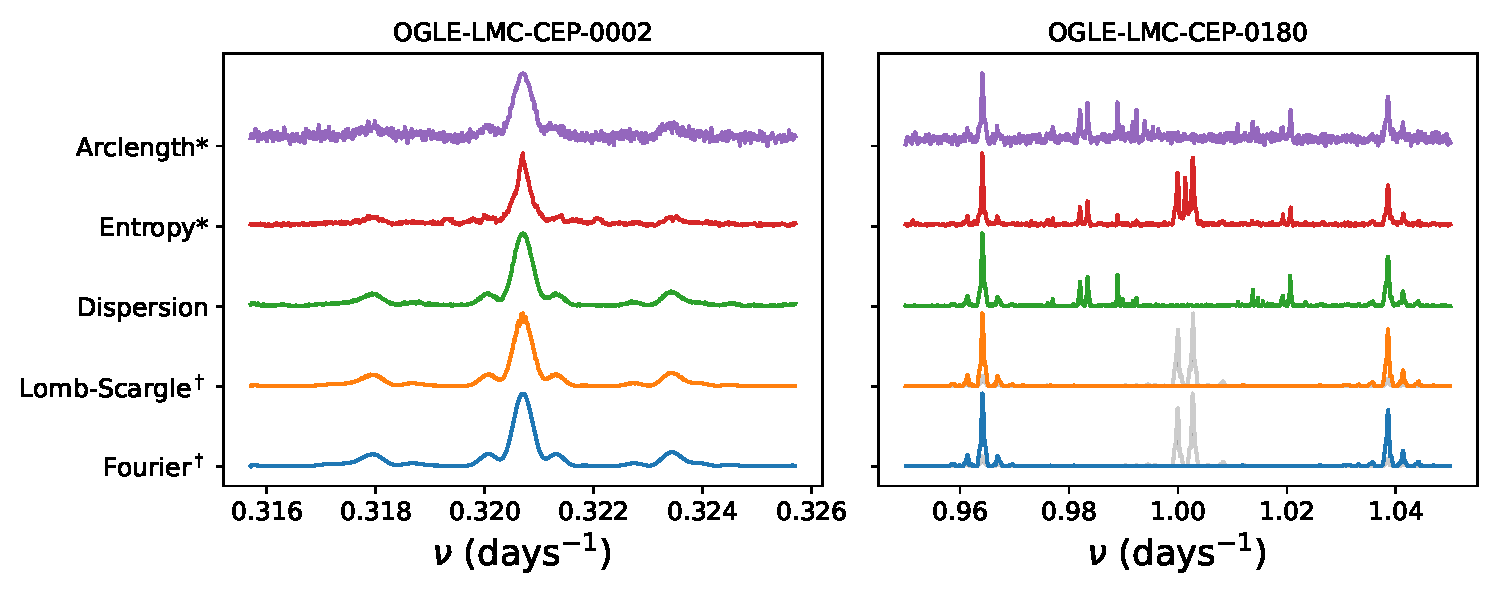
\includegraphics[width=0.99\textwidth]{img/examples.pdf}
	\caption[Example of spectra near the true frequency]{
		Sample spectra for the five methods described in this section, for two different stars, near the true frequency.
		$(\ast)$: Arclength and Entropy spectra were inverted to allow direct comparison with the Fourier approximations.
		$(\dagger)$: The Fourier, Lomb-Scargle and entropy methods present a false peak (in light gray) 
		when the frequency is very near 1/day; see text for details, and \autoref{fig:entropy-alias} for the behavior of the entropy false peaks.
	}
	\label{fig:examples}
\end{figure}

\begin{figure}
	\centering
	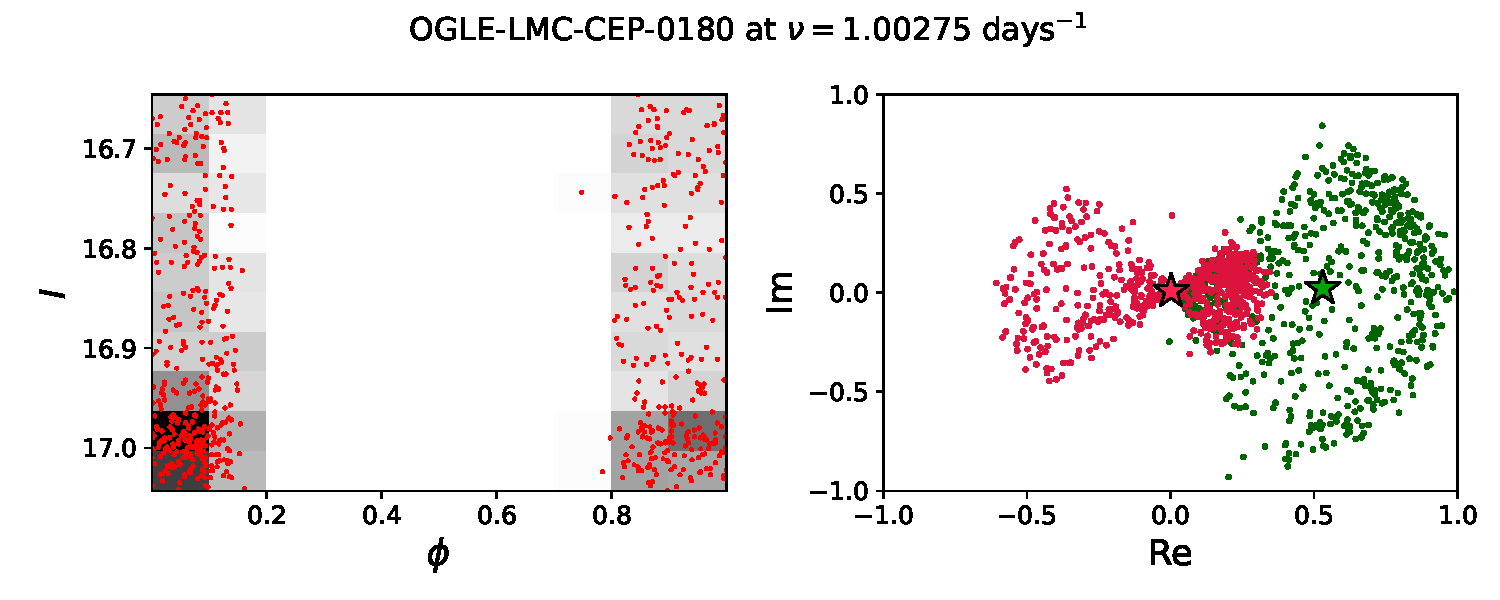
\includegraphics[width=0.8\textwidth]{img/alias.pdf}
	\caption[Detail of the failure mode of Fourier and entropy methods]{
		Detail of the phase diagram and complex phase curling of the star from \autoref{fig:examples}, very near the false peak at 1.00275/day.
		The histogram was made with 10 bins on each axis.
		The green and magenta dots represent a Fourier curling where the magnitude has been normalized in the respective intervals 
		$[0,\text{max}-\text{min}]$ and $[\text{min}-\text{mean},\text{max}-\text{mean}]$ (such that the mean becomes zero).
		The big stars lie on the centroid.
	}
	\label{fig:problem}
\end{figure}

Then is suddenly clear why the entropy method fails: the dots are distributed phase-wise in a similar fashion as in \autoref{fig:1234-cadence}.
That leaves a huge gap (in this case in the middle), and if there are many bins with probability zero the entropy would certainly be lower,
because it is more ordered that way; there are chunks of the phase diagram histogram that are uniform, and therefore the entropy method gives a false positive.
The specific behavior of these false peaks as a function of the number of zones is examined in \autoref{fig:entropy-alias}.

Something similar happens with the curled figure in the complex plane. As each point is rotated almost $360^\circ$ 
(again, how much more or less than that is dictated by \autoref{fig:1234-cadence}), and if the radii are all positive that means the centroid would be near the positive reals.
There is a simple solution: make the mean radius zero. That way, the negative radius would end in the $180^\circ$ side of the complex plane, and everything would cancel nicely.

\autoref{fig:problem} also allow us to understand how the arclength and dispersion spectra are \enquote{immune} to this effect. 
If we connect the dots of the phase diagram,  at least one line should join the two groups, and it will be a big line.
So no matter how close get those points on the sides, the big line between them should carry the weight of this strange alignment.
That works until everything aligns in one clump in the middle, and suddenly there is no line.
This could be corrected by connecting the $\phi=0$ and the $\phi=1$ points on the phase axis\footnote{
	This is like a quotient space in topology. The phase diagram is a square, and we join two edges, 
	and the result is a figure akin to the sides of a cylinder.
}, and considering also the arclength between the first and last point: 
auditioning a mixed term $\sqrt{(f_0'-f_N')^2+(\phi_0'-\phi_N')^2}$ to \autoref{eq:arclength}
would eliminate the possibility of central clumping; the points would be connected in a circular fashion.

On the other side, we defined the empty variance as zero. 
Therefore the terms corresponding at the empty gaps would just not contribute, neither in the denominator nor in the numerator of \autoref{eq:pooled-variance}.
It would be as if someone had just cut out the empty columns. The rest is just vertical chaos, having in fact maximal variance,
so the dispersion method is truly immune with our definitions.
 

%\section{Pulsation mode determination}

